\section*{Exercício 6}
\label{ex:6}
\addcontentsline{toc}{section}{Exercício 6}

    Para os critérios de projeto fornecidos, o projeto de controle será feito em espaço $s$ e o respectivo pólo deve pertencer ao lugar das raízes em malha fechada. O tempo de subida é dado por:
    
        \begin{equation}
            t^{0\% - 100\%}_{r}(\omega_n, \zeta) = \frac{\pi - \theta(\zeta)}{\omega_d(\omega_n, \zeta)} \mbox{, com } \theta(\zeta) = \tan^{-1}\frac{\sqrt{1 - \zeta^2}}{\zeta} \mbox{ e } \omega_d(\omega_n, \zeta) = \omega_n \sqrt{1-\zeta^2}
            \label{eq:tempo_de_subida}
        \end{equation}
    
    De mesma forma, o sobressinal é dado por:
    
        \begin{equation}
            M(\zeta) = e^{-\pi \frac{\zeta}{\sqrt{1-\zeta^2}}}
            \label{eq:sobressinal}
        \end{equation}
    
    Como (\ref{eq:sobressinal}) é bijetora, $\exists g(M) = \zeta \mbox{, } g: M \longmapsto g(M) \mbox{, } M \circ g (M) = M$. De fato $g(M) = \sqrt{\frac{\log^2{M}}{\pi^2 - \log^2{M}}}$. De mesma forma, para $\zeta$ fixo, analogamente, $\exists h(t_r) = \zeta\mbox{, }h: t_r \longmapsto h(t_r)\mbox{, } t_r(\zeta) \circ h = t_r$. De fato, $g(t_r) = \frac{\pi - \theta}{\omega_d(\zeta, t_r)}$. Por fim, $\forall s \in \mathbb{C}, \,\, s = \omega_n (\zeta + i \sqrt{1 - \zeta^2})$, logo a seguinte malha satisfaz os critérios estabelecidos em projeto
    
        \begin{equation}
        C(s) = K \frac{s + 0.7}{s + 2 \zeta \omega_n}
        \label{eq:Cs}
        \end{equation}
    
    O polinômio característico do sistema para \eqref{eq:Cs} em malha fechada é 
    
        \begin{equation}
        P(s) = s^2 + 2\zeta \omega_n + K \coloneqq 0
        \label{eq:polcarac}
        \end{equation}
    
    Ao considerar o projeto em tempo contínuo, utilizaremos a estratégia de cancelamento de pólo do controlador com o pólo da planta. Para o caso de cancelamento sem resíduo, o novo lugar das raízes permite que o pólo estabelecido pertença a este. Ademais, por inspeção, o polinômio característico \eqref{eq:polcarac} fornece o valor $K$ para os pólos em projeto i.e., $K = \omega_n^2$. Assim, a função de transferência fornecida é:
    
        \begin{equation}
            C(s) = \omega_n^2 \frac{s + 0.7}{s + 2 \zeta \omega_n}
        \end{equation}
        
    Para projeto de controle por meio da aproximação do mantenedor de primeira ordem por transformação de Padé, utilizaremos a fórmula de Padé de primeira ordem seguinte:
    
        \begin{equation}
        e^{x} \approx \frac{1 + \frac{x}{2}}{1 - \frac{x}{2}}
        \label{eq:pade}
        \end{equation}
    
    Desta forma, por meio de \eqref{eq:pade}, o segurador de ordem zero exato pode ser aproximado por
    
        \begin{equation}
        G_{zoh}(s) = \frac{1 - e^{-T_s s}}{s} \approx \frac{2}{ s + \frac{2}{T_s}}
        \end{equation}
    
    A fim de manter o ganho unitário da função de transferência acima, a aproximaçaõ será 
    
        \begin{equation}
        G_{zoh}(s) \approx \frac{\frac{2}{T_s}}{s + \frac{2}{T_s}} = \frac{1}{\frac{T_s}{2} s + 1} 
        \end{equation}
    
    A função de transferência em malha aberta do sistema é $G'(s) = C(s)G_{zoh}(s)G(s)$. De mesma forma ao projeto acima, o projeto de controlador em tempo discreto cancelará o pólo da planta com um zero do controlador. Para um controlador da forma \eqref{eq:controladorpade}, o pólo encontrado para projeto pertence a curva $1 + G'(s) \coloneqq 0$.   Com auxílio de software de manipulação numérica, encontramos $K$ e $p$ tal que o sistema satisfaça os critérios de  projeto. 
    
    A aproximação de Padé para o segurador de ordem zero no projeto do controlador aproxima o sinal em tempo discreto da ação contínua tanto para a ação de controle, saída e erro do sistema como representa as imagens \ref{fig:ex6controle}, \ref{fig:ex6saida} e \ref{fig:ex6erro}  respectivamente. Os diagramas de blocos utilizados para a simulação estão nas imagens \ref{fig:ex6continuo} e \ref{fig:ex6discreto}.
    
    \begin{equation}
    \label{eq:controladorpade}
        C(s) = K \frac{s + 0.7}{s + p}
    \end{equation}
    
    \begin{figure}[H]
	\center
	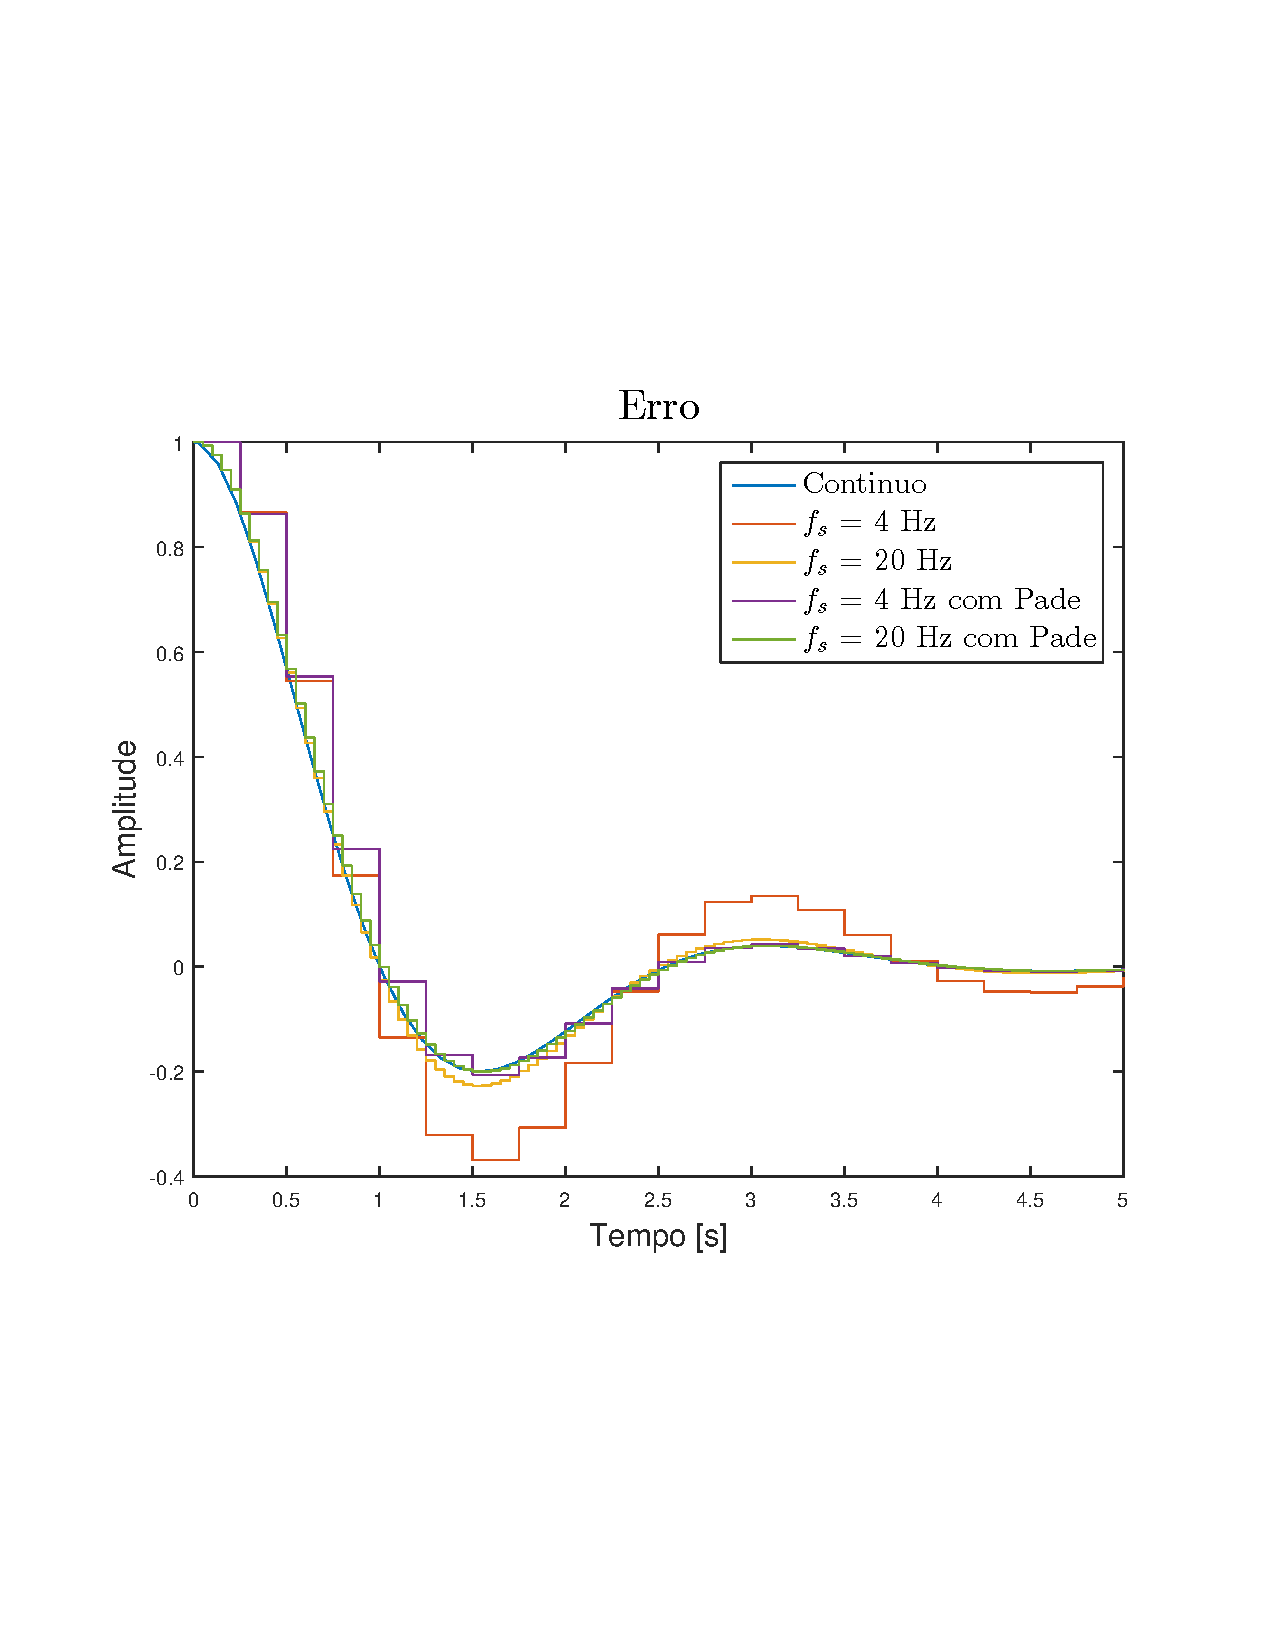
\includegraphics[width=0.8\textwidth]{controlezoh.pdf}
	\caption{Curva original e série amostrada}
	\label{fig:ex6controle}
    \end{figure}

\newpage

    \begin{figure}[htp]
	\center
	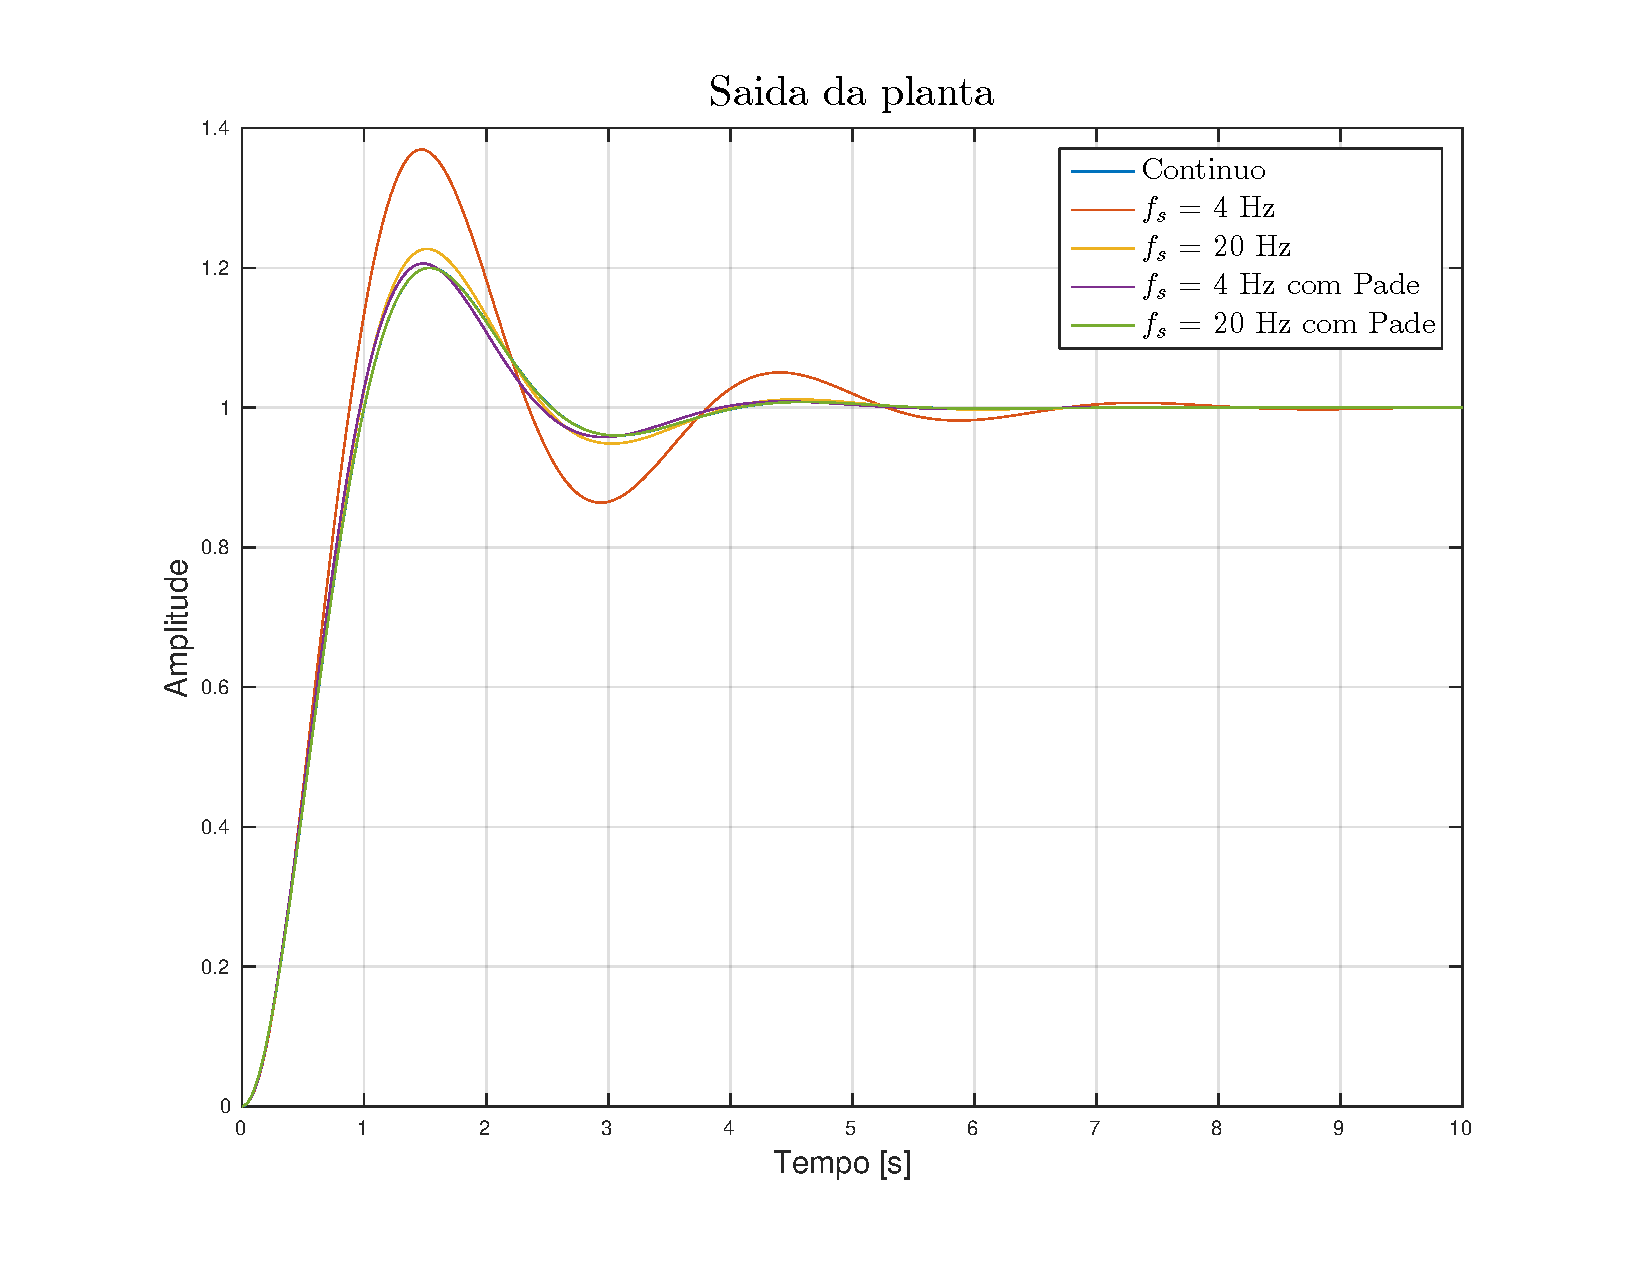
\includegraphics[width=0.8\textwidth]{saidazoh.pdf}
	\caption{Ação de controle para controle contínuo e discreto com $f_s = 4 Hz$ e $f_s = 20 Hz$. }
	\label{fig:ex6saida}
    \end{figure}

    \begin{figure}[H]
	\center
	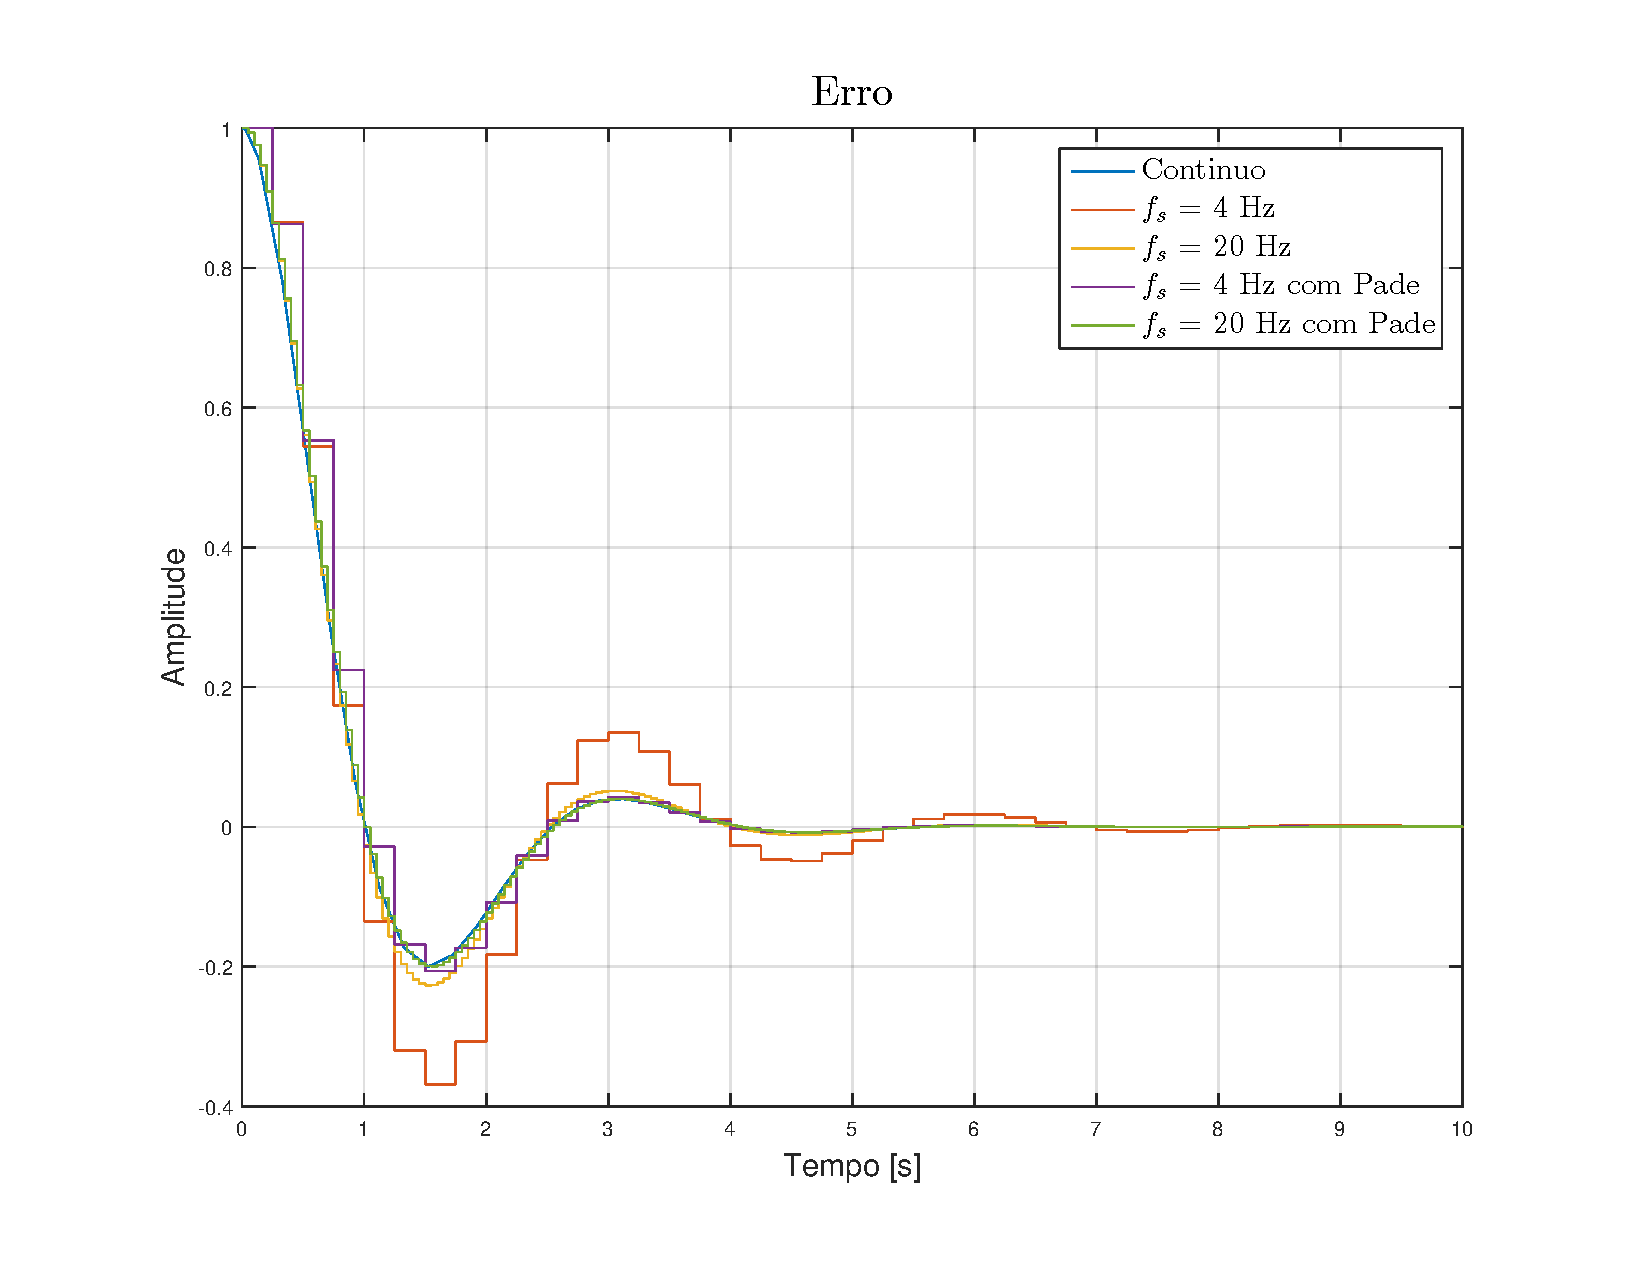
\includegraphics[width=0.8\textwidth, trim=3.5cm 2.5cm 2cm 2cm]{errozoh.pdf}
	\caption{Curva original e série amostrada}
	\label{fig:ex6erro}
    \end{figure}
    
    \begin{figure}[H]
	\center
	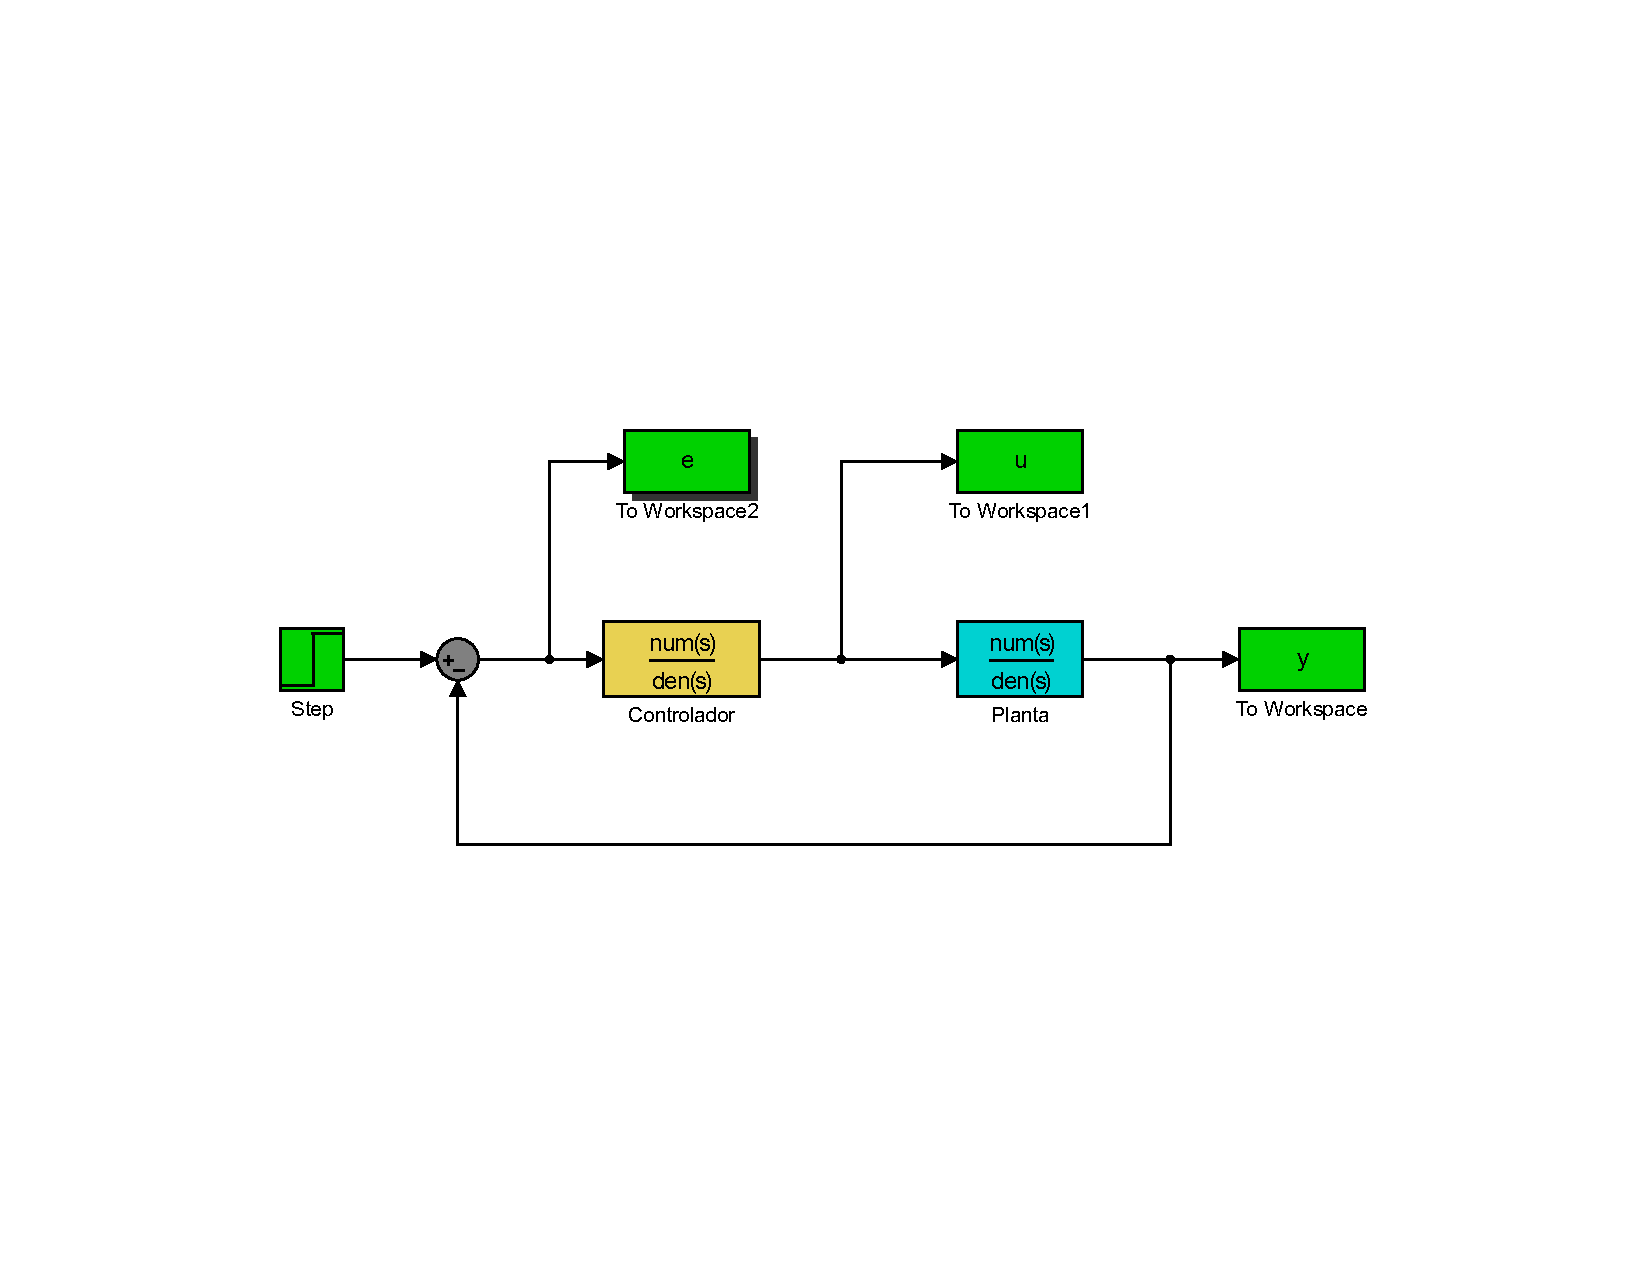
\includegraphics[width=0.8\textwidth, trim=3.5cm 2.5cm 2cm 3cm]{ex6simcontinuo.pdf}
	\caption{Diagrama de blocos em malha fechada com controle contínuo}
	\label{fig:ex6continuo}
    \end{figure}

    \begin{figure}[H]
	\center
	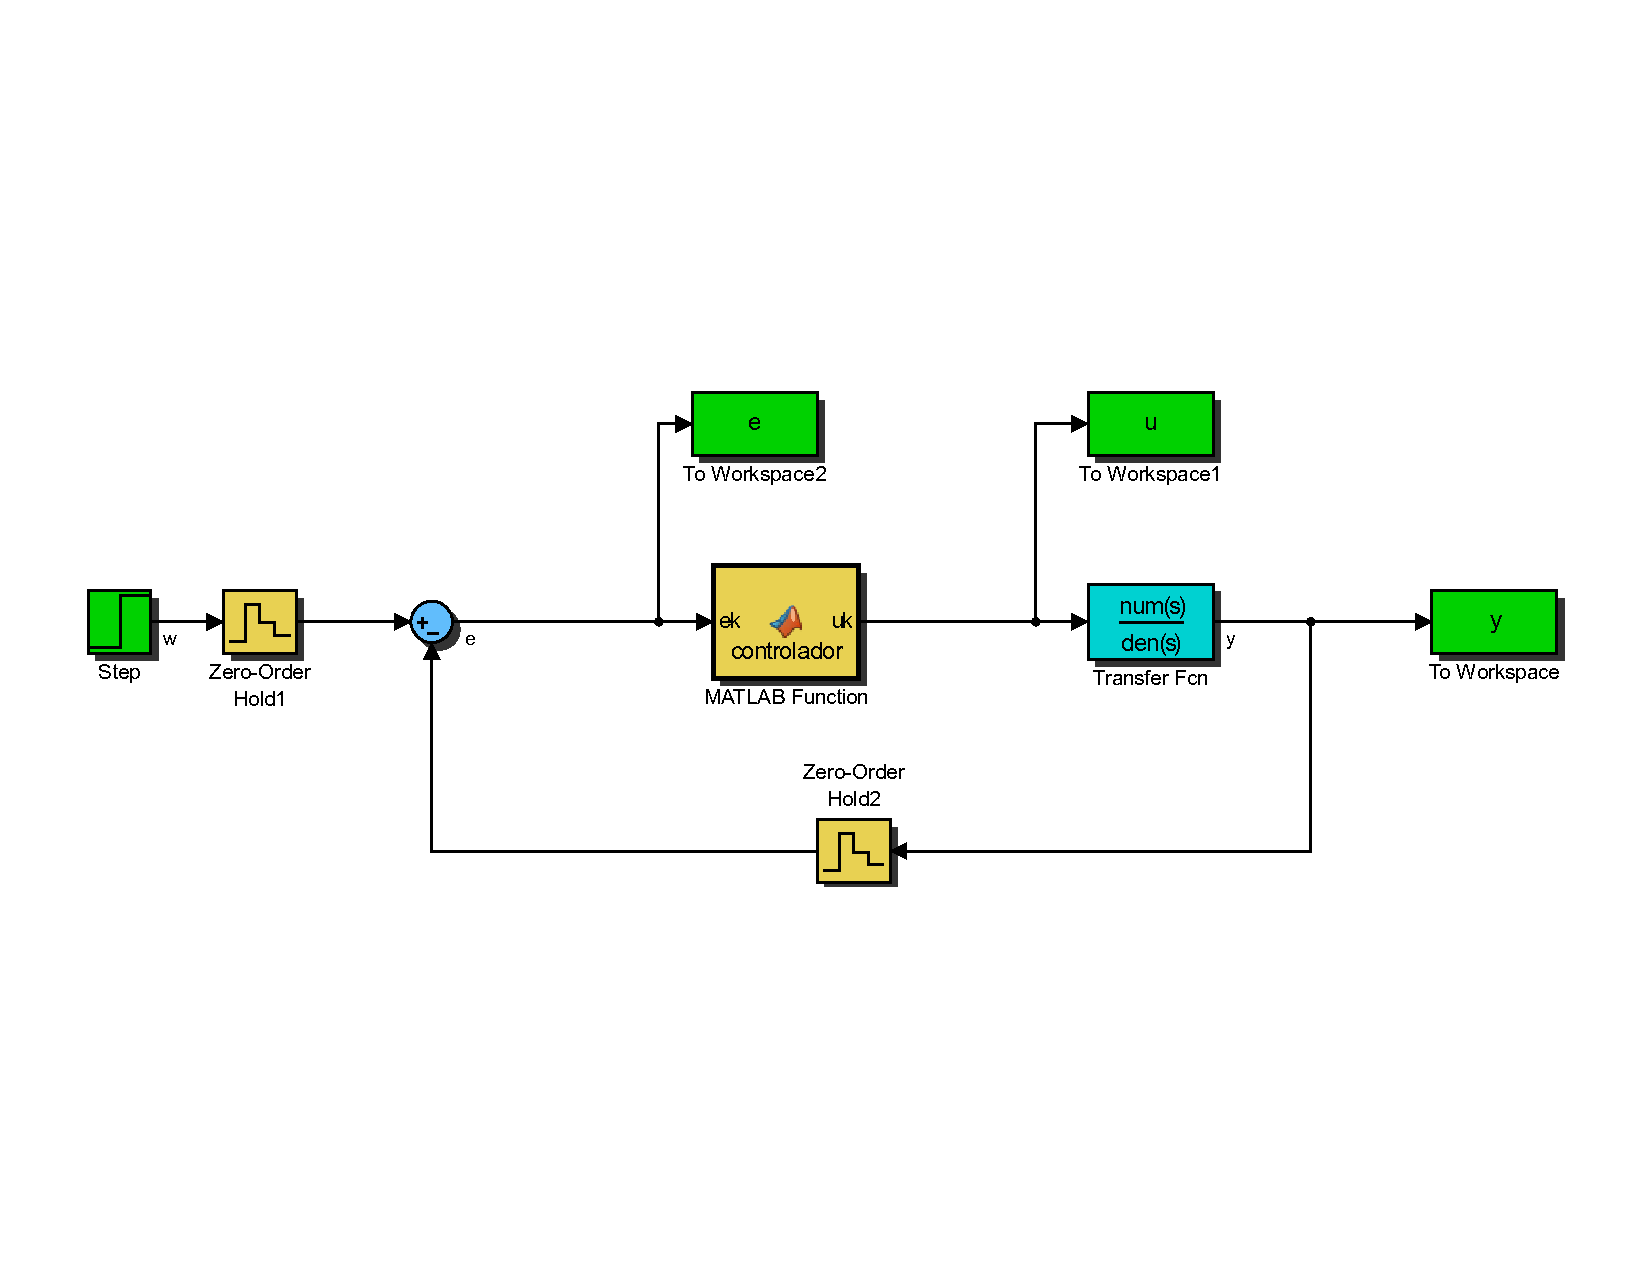
\includegraphics[width=0.8\textwidth]{ex6simdiscreto.pdf}
	\caption{Diagrama de blocos em malha fechada com controle discreto}
	\label{fig:ex6discreto}
    \end{figure}